% oneside to ensure no unnecessary blank pages are inserted and margins are equal across both odd and even pages.
\documentclass[oneside, whitelogo]{tudelft-report}

\usepackage{wrapfig}
\begin{document}
	
	%% Use Roman numerals for the page numbers of the title pages and table of
	%% contents.
	\frontmatter
	
	% Title and subtitle color can be configured by entering a colour as parameter for the subtitle command. 
	\title{Pantzerfaust\\DNav}
	\subtitle[tudelft-white]{Final Product Report}
	\author[tudelft-white]{
		W.\ Smit\\
		J.\ van der Krieken\\
		C.\ Athmer\\
		F.\ Elghlan\\
		C.\ Bilstra\\
	}
	\affiliation{Delft University of Technology} 
	\coverimage{cover.jpg}
	\titleoffsetx{1cm}
	\titleoffsety{6.5cm}
	\afiloffsetx{1cm} 
	\afiloffsety{18cm} 
	
	\makecover
	
	%% Include an optional title page.
	\begin{titlepage}
	
	\begin{center}
		
		%% Insert the TU Delft logo at the bottom of the page.
		\begin{tikzpicture}[remember picture,overlay]
		\node at (current page.south)[anchor=south,inner sep=0pt]{
			
\includegraphics{cover/logo}
		};
		\end{tikzpicture}
		
		%% Print the title in cyan.
		{\makeatletter
			\tudtitlefamily\color{tudelft-cyan}\fontsize{64}{94}\selectfont\@title
			%\largetitlestyle\color{tudelft-cyan}\Huge\@title
			\makeatother}
		
		%% Print the optional subtitle in black.
		{\makeatletter
			\ifx\@subtitle\undefined\else
			\bigskip
			{\tudsffamily\color{tudelft-cyan}\fontsize{22}{32}\selectfont\@subtitle}    
			%\titlefont\titleshape\LARGE\@subtitle
			\fi
			\makeatother}
		
		\bigskip
		\bigskip
		
		by
		%door
		
		\bigskip
		\bigskip
		
		%% Print the name of the author.
		{\makeatletter
			%\largetitlefont\Large\bfseries\@author
			\tudtitlefamily\color{tudelft-black}\fontsize{26}{26}\selectfont\@author
			\makeatother}
		
		\bigskip
		\bigskip
		\bigskip
		
		\begin{tabular}{llll}
			\multicolumn{4}{l}{Student numbers:}\\
			
			Wouter Smit & 4401409 & Faris Elghlan & 4341538\\
			Justin van der Krieken & 4357116 & Cas Bilstra & 4381084\\
			Casper Athmer & 4329066 &\\
			
			\\
			\multicolumn{2}{l}{Project duration:} & \multicolumn{2}{l}{April 18, 2016 -- June 23, 2016} \\
			\multicolumn{2}{l}{Context coordinator:} & \multicolumn{2}{l}{Thomas Abeel} \\ 
			\multicolumn{2}{l}{Customer representative:} & \multicolumn{2}{l}{Thomas Abeel} \\ 
			\\
			\multicolumn{2}{l}{Teaching Assistants:} & \multicolumn{2}{l}{Sjoerd Huisman}\\
			\multicolumn{2}{l}{} & \multicolumn{2}{l}{Jasper Linthorst}\\
			\\
			\multicolumn{2}{l}{Software Teaching Assistant:} & \multicolumn{2}{l}{Jim Hommes}\\
		\end{tabular}
		
		%% Only include the following lines if confidentiality is applicable.
		\bigskip
		\bigskip
		\emph{}
		%\emph{}
		
		\bigskip
		\bigskip
		
	\end{center}
	
\end{titlepage}
	
	\tableofcontents
	
	%% Chapters are separated into files. 
	
	%% Use Arabic numerals for the page numbers of the chapters.
	\mainmatter
	
	\chapter{Introduction}
\par
Tuberculosis is a big problem in modern society. It’s a deadly disease (if untreated, the disease kills about half of those infected) and about one third of the world population is infected with it \citep{whoTB}. Curing this disease takes at least six months with the current medicines and possibly up to three years in which six variants of antibiotics have to be taken\citep{p1TB}.
\par
Drug-resistant tuberculosis is becoming an increasingly difficult problem. Research is being done in order to make new vaccines, drugs and diagnostics to improve the ability to cure this disease. One of the institutes performing this research is the Broad Institute, an institute for biomedical science, which is being run by MIT and Harvard. To do this research efficiently, an application to compare and visualize multiple DNA sequences (genomes) is needed. Last year an attempt was made by students from the Delft University of Technology, but the applications they created did not suffice. The main problems were that programs were not scalable (they could only load a small dataset of genomes) and missed semantic zooming. This year the development project is repeated. This report describes the development of such an application, which can help biologists explore Tuberculosis genomes.
\par
The goal for this application is to create a tool for interactive visualization of DNA sequence graphs to enable exploratory data analysis. The application must comply with the following requirements:
\begin{itemize}
	\item The visualization must be interactive (i.e. the user should be able to easily navigate the visualization).
	\item Semantic zooming. The customer expects to be able to zoom in onto the visualization. As the visualization is more zoomed in, more information should become visible.
	\item Integration between phylogeny (i.e. ancestral history of genomes) and the genomes. Usually represented as a tree. Such tree could be used as navigation device.
	\item Metadata about genomes and annotations of parts of (the reference) genome should be integrated. Ideally these should be easily accessible (e.g. searchable).
\end{itemize}

Lastly, the customer would like to be able to detect a phenomenon called convergent evolution. This occurs when two two separate branches of the evolution of the genome separately mutated in the same way. This indicates that this mutation is likely to happen evolutionary, regardless of previous mutations of a genome.

	\input{chapters/OverviewOfThefinalProduct}
	\chapter{Reflection on the product and development process (SEM)}
This section evaluates the development process of the product and the technical aspects of the product. The evaluation of the development process includes evaluating the dynamics in the group, the use of sprints and the documentation. Evaluating the technical aspects of the project focuses on the quality of the code. 

\section{Development process}
\par
The dynamics in the group were good. The communication in the group went through different channels, including e-mail, WhatsApp, Slack, GitHub, and face-to-face. In retrospect, it would have been better to have less channels of communication, because checking all aforementioned channels is cumbersome. However, during this project the high number of communication channels did not cause problems. 
\par
During this project, a new sprint planning was made weekly. This was not ideal, because a sprint of a week is short, and there have been big tasks which take longer than a week, which are therefore hard to put in a sprint planning. 
\par
The sprint plannings that have been made also tended to include too much work for a week. Often, the development of new features took longer than was accounted for in the spring planning, which meant not all tasks on the planning were done. For future projects, it’s important to better estimate the time it costs to develop new features.
\par
The formal documentation during this project included an Architecture Design, the weekly sprint planning and sprint retrospective. This documentation has not been used by any member of the group during the development phase. A useful form of documentation were the issues on GitHub. These were used extensively, and showed a nice overview of tasks to be done. 

\section{Product evaluation}
\par
The code for the application has been split in modules. A big advantage of this is that a module can be taken out and replaced with another module, without changing the rest of the code. The use of modules brought challenges with it (e.g. the visibility of classes), but is a nice way to separate code. 
\par
An important principle which has been used a lot, is the use of interfaces. The model classes have all been implemented using an interface, which makes it more reusable. 
A part of the program which is not as reusable, is the GUI part. Some of the classes in this module have become large, which is inherent to using JavaFX\footnote{http://docs.oracle.com/javase/8/javafx/get-started-tutorial/jfx-overview.htm}. Another reason that this happened, was the fact that the client demanded many new features every week. There is a constant tradeoff to be made between quality of code and the quality of the program (in terms of features). During this project the latter was often preferred.
	
\chapter{Description of the developed functionalities}
This chapter will give a description of the functionalities that are developed for our application. The requirements mentioned in the introduction are used to reflect on the functionalities.
\section{Semantic zooming}
\begin{wrapfigure}{r}{0.2\textwidth}
	\centering
	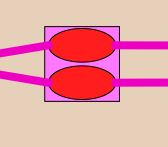
\includegraphics{images/mutation.jpg}
	\caption{\label{fig:bubble}A mutation bubble}
\end{wrapfigure}
Semantic zooming should be provided to the customer which initially shows the entire graph, and on which the user can zoom in to see more details. This is implemented by making bubbles, which collapse nodes together, and showing these at a high-level view. When zooming in (which happens stepless), the bubbles are expanded and more details of the graph are shown. By creating bubbles, large amounts of genomes can be visualized. When nodes in the graph (which represent base sequences) are big enough they become visible. Figure X+1 shows an example of a bubble (the purple square), containing two nodes, which has been expanded. 

\section{Phylogenetic tree}

\begin{wrapfigure}{l}{5cm}
	\centering
	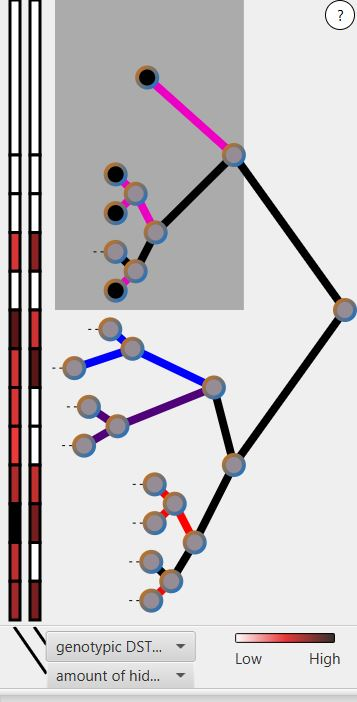
\includegraphics[width=0.3\textwidth]{images/tree.jpg}
	\caption{\label{fig:tree}The phylogenetic\\tree}
\end{wrapfigure}

The phylogenetic tree can be used to visualize a subset of the genomes. The tree in the application can be zoomed in on, because not every leaf node can be shown on the screen when the dataset is big. By zooming in, nodes on a deeper level become visible. 
\par
There exist lineages in the phylogeny, which is a grouping of genomes. These lineages have a specific colour which is shown on the edges between nodes in the tree. 
\par
On the left of the tree is a heatmap which can be used to show the density of properties of the tree (e.g. the number of leaf nodes in a certain branch). 
\par
Nodes can be dragged from the phylogenetic tree to the main graph area and all genomes contained in the leaves of the selected tree are then drawn on the screen. When dragged to the main area a popup will appear asking if the genomes should be added to the existing graph, if a new graph has to be created, or if the specific nodes have to be removed from the current visualization. 
\par
Because the application builds on the idea that the comparison of two graphs can be useful, two graphs can be drawn on the main screen. Nodes in the tree have colouring to indicate in which graph(s) they are present. There is a legend present for all visuals in the tree. 
Figure X+2 shows an example of the phylogenetic tree, with one heatmap containing the amount of hidden nodes in a branch and the other heatmap containing the amount of genotype DST:XDR in a branch.
\section{The main area}
The main area is the part where the graph is drawn. As mentioned before, there can be a graph on the top half and a graph on the bottom half (see figure X). It is also possible to show only one graph. Loading is performed with simple dragging and dropping from the phylogenetic tree. When a graph is loaded, the user sees different rectangles, ellipses, and colours. These represent different types of bubbles, which are explained in the legend. 
\section{Searching}
On the main screen a searching pane is available. A search can be performed based on metadata about the genomes. Multiple genomes that resulted from a search can be selected and dragged to the main graph. This works the same as dragging and dropping from the phylogenetic tree.
\section{Loading}
When the application is started a file loader appears wherein the files to be loaded can be selected. The application supports the .gfa file-format for the graph, the .nwk file-format for the phylogenetic tree, the .gff file-format for the annotations and the .xlsx file-format for the metadata. 
\section{Settings}
There is a settings menu, where the user can select which bubbling algorithms it wants to use (if any). There are five options to choose from, which are explained in the application.
	
	\chapter{Human-Computer Interaction Design}
The application is highly complex because of the nature of the application and its many functionalities.To assert the quality of interaction with the user and to detect flaws in the interaction design, an experiment has been conducted that tests the users’ ability to find and use the features of the application to correctly and easily derive conclusions.

\section{Method}
In this section a description can be found on what the experiment consists of and how the experiment should be performed, in such a way that the result should be reproducible.

\section{Target}
The goal of the experiment is to assert the test users’ ability to intuitively understand the graphical user interface and, in particular, understand the representation of the research data that is used in the application.

\section{Procedure}
The experiment will consist of two stages. In the first stage, the participants are shortly trained in the basic biology principles necessary to understand the tasks they are given, as well as explained what the data is and what it represents.
In the second stage, the participants spend 15 minutes performing a small list of tasks inside the application, which mimic the expected research questions that the end-user may have. This stage is executed individually with the researcher.
In the third stage, the test users are interviewed to reflect on their experience and the problems they encountered while using the application.

\par
The following tasks as set on the user. Each task is provided after the previous has been finished.

\begin{enumerate}
	\item Produce the sequence graph of the complete data set.
	\item Find the position of the gene ‘katG’ in the DNA.
	\item Decide if there are any mutations in the gene.
	\item If any mutations are present, find out what nucleotides differ between the mutations.
\end{enumerate}

\section{Tasks}
This usability test should be performed by at least 2 persons: the researcher and the participant. Because the whole test will be captured there is no need for more than one person to analyse the user, as the researcher can have another look at the experiment afterwards.
\section{Measurement}
The duration of each task is measured and the researcher takes notes of interactions that take significantly longer than expected. If the participant takes longer than the maximum amount of time to complete one of the tasks, the researcher provides a hint to steer the participant towards the answer. This signifies that the participant was not able to find the functionality required to complete the task autonomously. This can point to certain aspects of that task being unclear, unavailable, or insufficiently useful.
\par
In addition, the tasks that require the participant to derive a conclusion, are marked correct or incorrect.

\section{Participants}
The test users are currently students in biology related areas, such as medicine or (micro)biology. These backgrounds provide general understanding of DNA and proteins, but not necessarily about the bioinformatical aspects of DNA sequencing and sequence alignment. This knowledge is provided during the training.
\section{Result}
We provide the results of the measurements for each step in appendix \ref{ch:human-computer-interaction-design-results}. 
\par
The results show that especially finding the gene was a very hard task to the participants. In the majority of the time, they required a hint to know how to do this. After this, the last two tasks were easier than expected, requiring on average way less time. The last task was completely accurately performed, although the task of detecting a mutation sometimes led to wrong conclusions. The first task yielded expected results.
\par
The notes describe a few recurring events of confusion. Firstly, the coordinate system displayed in the scrollbar is a different system than the gene annotation coordinates. Participants tried to scroll to the location, but could not find the gene at the supposedly correct location. In order to find the gene, participants tried typing the name of the gene in the field where a base number can be chosen to jump to. Lastly, when participants clicked on the gene in the gene list, the jump did not trigger because they were fully zoomed out, therefore making it unclear that they could directly jump to them.

\section{Discussion}
We see from the results that the task of locating a gene was perceived as rather hard. Most participants required a hint to be able to do this. The experiment notes describe a lot of confusion about the search tools, either using them for the wrong purpose, or using the right tool but without the desired outcome. After the hint, all participants were able to instantly solve the task, showing that the tools and functionality works sufficiently, but the simplicity is suboptimal.
\par
All tasks can be completed within a total time of 1 minute, if done by an experienced user, i.e. a user who knows what every functionality does and has sufficient biological background. The participants could perform these steps afterwards as well within similar time, after being receiving the hints for every task.
\par
This is also in line with the last two tasks: as soon as participants had found the actual gene, the application provided sufficient information to understand mutational patterns in the data.

\section{Conclusion}
We conclude that the application has all functionality that is required to perform tasks very quickly and efficiently, however, the usage of these features are not intuitive enough to be understood by the user without the current amount of explanation.
\par
Because of this, we can expect that a short training, or additional tutorials or introductory features will improve the learning curve.
\par
We also note that participants were generally able to interpret the data correctly, even with limited biological knowledge. This means that users who are experts in this field of biology should be even more able to do so. 
\section{Imperfections in Methodology}
The experiment has a few flaws, which we will discuss for future improvement.
Firstly, the participants were only partially representative of actual end users. They have no knowledge of the data set and what possible mutations are or could mean. They are not familiar with all jargon. All these aspects hinder in their intuitive knowledge of the application.
Secondly, the measurement for the first task included the participants’ first impression of hte application. The measured time included more than solely the task and therefore came out higher than expected.
Lastly, the experiment does not cover the learning curve, although we do expect that this will have an effect. To more firmly establish this claim, the experiment should be repeated with participants that are shortly introduced to the application, so that their results can be compared against untrained participants.
\section{Recommendations}
We finish with recommendations about the interaction design of the application.
\par
Firstly, we suggest that the jumping features also zoom in on the graph, so that the user will directly see the desired element, regardless of the current zoom level.
\par
Secondly, we suggest that the application is extended with a form of help, which can be in the form of introduction steps that describe the process of using the application, or with additional information that is shown per element in the application. We note that personal training is most likely the most effective strategy, although this might be not always possible.

	
	\chapter{Evaluation of the functional modules and the product in its entirety, including the failure analysis}
To evaluate the functional modules and the product in its entirety, the feedback given by the client about the program is used. The program is made for the client which means that their feedback is most valuable in evaluating the program. The evaluation of the developers is also used for evaluating the program, because the developers know in which areas the program can improve. 

\section{Program evaluation}
Overall the application that is built is good. It meets the wishes of the client and has an extensive list of features. There are issues in the application which have not been solved. These are discussed below.
\subsection{Vertical spacing}
The fact that the client didn’t want vertical scrolling (i.e. all nodes in the vertical spacing are shown on the screen), caused nodes to be barely visible in locations with many branches. One way to solve this would be to add the ability to also zoom vertically, but this was something which was not desirable for the client at this time. Another option would be to use the vertical space more efficiently and to make the nodes smaller.

\subsection{Usability of the program for biologists}
In terms of speed the program has an outstanding performance, which makes it usable. However, the program has a lot of features, which can be overwhelming for a user.The program needs guidelines for a user to be able to use it. 
Another issue with usability relates to the problem of vertical spacing. Because of this problem, more complicated structures in the graph can be not be explored. 
A big issue for the biologists was finding convergent evolution, and our program can still improve in this area. There is some visual help in finding convergent evolution with the phylogenetic bubbles, but it’s open to improvement.  Highlighting convergent evolution in the graph would be a huge improvement. 


	\chapter{Outlook}
In this section, improvements that can be made for this product are discussed. This can be useful for further development of this application, or the development of a new application with the same purpose. Even though the time to build the program was limited, the application satisfies the client and is considered finished. There are points of improvement, which are discussed below.
\par
The biggest dataset that was available to run the program with, contained 328 genomes. Loading this graph takes 3-6 seconds, which is quick. There is a dataset containing 6000 genomes, which indicates a highly complex graph. Rendering this graph will take a lot longer, and it might also cause memory issues because everything is saved in main memory currently. A way to solve these problems is to use a dataserver with which the application communicates. This solves the problem of using too much memory. Using a remote dataserver it is possible to precompute big parts of the graph, which can increase the loading time. Concluding, adapting the application to work with a remote dataserver makes the application more scalable.
\par
In the current application, when the graph with 328 genomes is drawn, it’s impossible to explore parts of the graph with many branches. The reason for this is that there isn’t enough vertical space, which causes the nodes to become almost invisible. The ability to zoom vertically can solve this problem. 
Finally, an improvement to the program would be highlighting of convergent evolution. Convergent evolution is a phenomenon which can be useful for biologists, so highlighting it would increase the value of the program for biologists.
\par
Concluding, there are areas in which the program can make steps to improve. Within a timespan of 10 weeks the developers managed to build a program which is appreciated by the client, and which forms a solid foundation for further development of tools to visualize DNA sequences. 

	
%	\input{chapters/ProgramOfRequirements}
	
	\bibliographystyle{apalike}
	\bibliography{report}
	
	%% Use letters for the chapter numbers of the appendices.
	\appendix
	\input{appendices/appendices}
	\addcontentsline{toc}{chapter}{Appendices}
	
	\chapter{Human-Computer Interaction Design Results}
\label{ch:human-computer-interaction-design-results}

If the maximum time was reached, we implicitly assume that the hint was given and the participant continues on to the next task. The results for each task are not listed per participant, for sake of anonymity.

\begin{center}
	\begin{tabular}{| l | l |}
		\hline
		\multicolumn{2}{|c|}{Loading the graph} \\
		\hline
		Participant & Time spent\\
		\hline
		1 & 01:47\\
		2 & 01:34\\
		3 & 00:54\\
		4 & 02:03\\
		5 & 03:00\\
		\hline
		Average & 01:52\\
		\hline
	\end{tabular}
\end{center}

\begin{center}
	\begin{tabular}{| l | l |}
		\hline
		\multicolumn{2}{|c|}{Finding gene ‘katG’} \\
		\hline
		Participant & Time spent\\
		\hline
		1 & 07:00\\
		2 & 05:34\\
		3 & 07:00\\
		4 & 07:00\\
		5 & 04:22\\
		\hline
		Average & 06:29\\
		\hline
	\end{tabular}
\end{center}

\begin{center}
	\begin{tabular}{| l | l | l |}
		\hline
		\multicolumn{3}{|c|}{Deciding whether there are any mutations within the gene} \\
		\hline
		Participant & Time spent & Conclusion\\
		\hline
		1 & 00:29 & Correct\\
		2 & 00:13 & Incorrect\\
		3 & 00:44 & Incorrect\\
		4 & 00:58 & Correct\\
		5 & 00:24 & Correct\\
		\hline
		Average & 00:34 & 60\% Correct\\
		\hline
	\end{tabular}
\end{center}


\begin{center}
	\begin{tabular}{| l | l | l |}
		\hline
		\multicolumn{3}{|c|}{Finding out what nucleotides form the mutation} \\
		\hline
		Participant & Time spent & Conclusion\\
		\hline
		1 & 00:24 & Correct\\
		2 & 00:54 & Correct\\
		3 & 00:11 & Correct\\
		4 & 00:12 & Correct\\
		5 & 00:21 & Correct\\
		\hline
		Average & 00:24 & 100\% Correct\\
		\hline
	\end{tabular}
\end{center}
	
	
	% All references should be in the bibliography, even when not cited in text.
	\nocite{*}
	
\end{document}